\documentclass[a4paper]{article}

\usepackage[english]{babel}
\usepackage[utf8]{inputenc}
\usepackage{amsmath}
\usepackage{graphicx}
\usepackage[colorlinks,linkcolor=blue]{hyperref}
\usepackage[colorinlistoftodos]{todonotes}
\usepackage[noindent]{ctex}
\usepackage{amsmath}
\usepackage{lipsum}
\usepackage{color}


\title{\Huge \heiti{操作系统实验(二)}}

\author{\lishu{南京大学软件学院}}

\date{\normalsize 2015.4}
\begin{document}
\maketitle

\renewcommand{\abstractname}{实验重点}

\begin{abstract}
本次作业重点:熟悉掌握Fat12文件系统,$gcc+nasm$联合编译实践以及了解实模式与保护模式的基本内容。
\end{abstract}

\section{实验内容}
\subsection{编程读取FAT12文件}
~~~~~~编写程序read\_fat12,读取a.img文件(该文件是fat12文件系统的软盘镜像)。
\begin{itemize}
	\item 通过分析fat12文件系统,打印出所有文件。
	\item 打印完成后,要求能够获取用户输入文件路径(以回车结束),程序查询Fat12文件,分别对目录文件、普通文件、不存在的文件进行做相应的输出,具体规则见下文描述。
\end{itemize}

\subsection{输入输出示例}
~~~~~~比如对于如下目录结构的一个文件:
\begin{figure}[htbp]
\centering
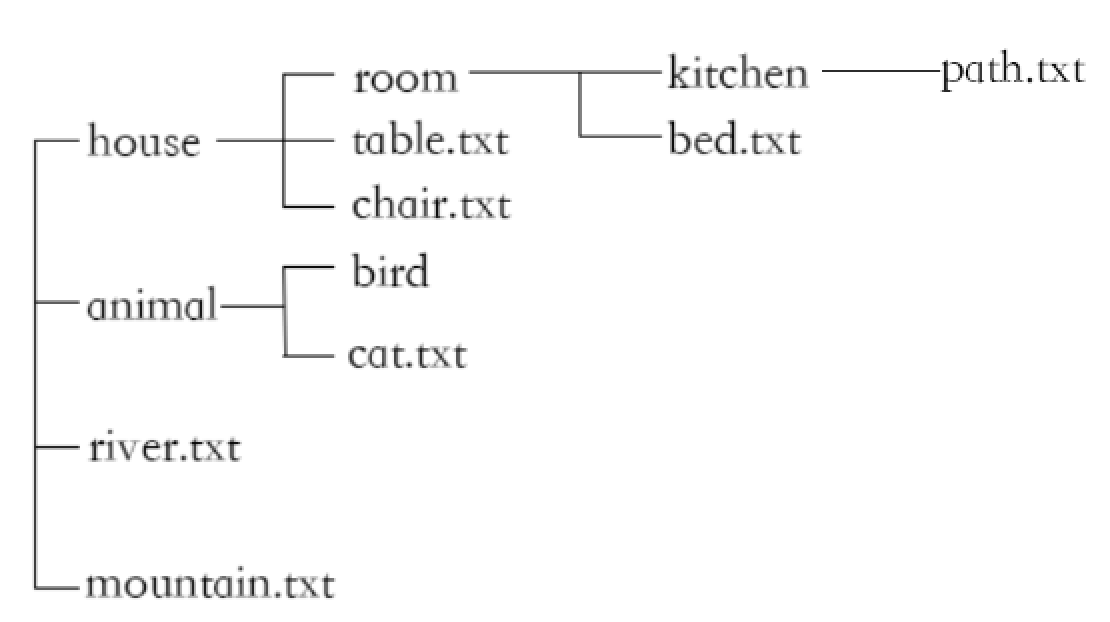
\includegraphics[width=0.7\textwidth]{path.png}
\end{figure}

\begin{itemize}
	\item 第一步的输出应该为:
	
\fbox{%
  \parbox{\textwidth}{%
    \begin{minipage}{\textwidth}
      {\color{blue}{house/room/kitchen/}}path.txt
      
       {\color{blue}{house/room/}}bed.txt
       
        {\color{blue}{house/}}table.txt
        
        {\color{blue}{house/}}chair.txt
        
        {\color{blue}{animal/bird}}
        
         {\color{blue}{animal/}}cat.txt
         
         river.txt
         
         mountain.txt
    \end{minipage}
  }%
}


	\item 第二歩的输入输出与下例类似:
	\begin {itemize}
		\item 输入“house/room/”,显示如下内容:
		
		house/room/kitchen/path.txt
		
		house/room/bed.txt
		\item 输入“house/room/bed.txt”,而bed.txt里面的内容是“Person”,显示如下内容:
		
		Person
		\item 输入“house/room/beeeed.txt”,显示如下内容:
		
		Unknown file
	\end {itemize}
\end{itemize}

\subsection{注意事项}
\begin{itemize}
	\item 注意是直接根据fat12文件系统格式直接读取a.img中的二进制内容,请不要先调用系统命令将a.img挂载再去调用系统命令遍历文件夹。
	\item 只需要支持纯英文字符即可,不用考虑中文文件名。
	\item 请将目录和普通文件用不同的颜色输出(不用按照示例输出中的颜色)。
	\item 程序只需要考虑接受一条输入,显示一条结果即可,不用考虑退出问题。
	\item 输入文件路径以回车符号结束,要求可以多次不断输入。
	\item 检查时会\underline{检查代码},可能的考察方式包括:
	\begin{itemize}
		\item 要求进行.img文件的挂载,删除目录或文件,重新运行程序,即改变输入。
		\item 要求对代码稍作修改后,比如对颜色等,重新make运行。
	\end{itemize}
	\item 要求程序由两个源文件构成,\textbf{main.c}和\textbf{my\_print.asm},其中main.c是主程序,可以使用基本的C库。但是打印不能使用标准函数printf,要求使用my\_print.asm中使用汇编编写的
	my\_print函数。
	\item 要求使用makefile编译链接两个文件,并作为作业的一部分提交。(如果是使用mac平台或者windows平台的同学请额外加txt文件说明下,其他同学默认使用linux平台)
\end{itemize}

\subsection{补充说明}
~~~~~~由于保护模式不容易理解,而且代码也比较死,所以这次代码作业没有去写保护模式的 代码,而是探究了操作系统中的“文件系统”这一主题,正好 loader 部分也涉及到对 fat12 的理解。

同时 gcc 和 nasm 联合使用也是为之后的实验奠定基础。

\subsection{链接实验}
~~~~~~按照链接相关PPT中要求完成动态链接实验的同学可以获得加分。注意,必须通过实验手段验证每一步并进行解释,参照PPT中静态链接相关内容。

请提供你的实验过程截图,使用的所有源代码,将其组织成报告提交到TSS。检查时请向助教主动演示,并回答助教的随机提问。

提示:可以使用PPT中的代码和PPT上提示的命令。


\section{问题清单}
~~~~~~在整个实验的过程中,无论是编程还是查资料,请各位同学注意思考以下问题,助教检查时会从中随机抽取数个题目进行提问,根据现场作答给出分数。
\underline{请注意,我们鼓励自己思考和动手实验},如果
能够提供自己的思考结果并辅助以相应的实验结果进行说明,在分数评定上会酌情考虑。

\subsection{PPT相关内容}
\begin{enumerate}
	\item 实模式下的寻址方式以及实模式的缺陷
	\item 保护模式下的寻址过程:
	\begin{itemize}
		\item 段寄存器中存储的是什么?GDT 是什么?LDT 是什么?如何区分 LDT 和 GDT? LDT 和 GDT 的区别是什么?如何定位到 Descriptor?Descriptor 的内容有哪些?
		\item GDTR 中的内容是什么?LDTR 中存储的是什么?为什么 LDT 要放在 GDT 中?
	\end{itemize}
	\item 选择子的作用:
		\begin{itemize}
			\item 选择子是什么?它的值存放在哪里?
			\item 选择子里面的内容有哪些?
			\item 为什么偏移地址大小是13位?
		\end{itemize}
	\item 描述符的作用:
	\item GDTR/LDTR 的作用:
		\begin{itemize}
			\item GDTR的内容是什么?
			\item LDTR的内容是什么?
		\end{itemize}
	\item 根目录区大小一定么?扇区号是多少?为什么?
	\item 数据区第一个簇号是多少?为什么?
	\item FAT 表的作用?
	\item 解释静态链接的过程。
	\item 解释动态链接的过程。
	\item 静态链接相关PPT中为什么使用ld链接而不是gcc。
	\item linux下可执行文件的虚拟地址空间默认从哪里开始分配。
\end{enumerate}

\subsection{实验相关内容}
\begin{enumerate}
	\item BPB 指定字段的含义
	\item 如何进入子目录并输出(说明方法调用)
	\item 如何获得指定文件的内容,即如何获得数据区的内容(比如使用指针等)
	\item 如何进行 C 代码和汇编之间的参数传递和返回值传递
	\item 汇编代码中对 I/O 的处理方式,说明指定寄存器所存值的含义
	\item 可以要求解释某些看不懂的代码(我看不懂的话,你得讲给我听)
\end{enumerate}

\section{参考资料}
	\begin{enumerate}
		\item 《Orange'S:一个操作系统的实现
		\item \href{http://jingliu.me/my_files/nasm.pdf}{Introduction to NASM}
		\item \href{http://www.eit.lth.se/fileadmin/eit/courses/eitn50/Projekt1/FAT12Description.pdf}
		{An overview of FAT12}
		\item \href{http://www.iecc.com/linker/linker10.html}{Dynamic Linking and Loading}
	\end{enumerate}

\end{document}
